% !TeX root = ../main.tex
\section{Radar Pasywny}
\label{sec:passive_radar}

% ------------------------------------------------------------------------
% Rozdział 2: Podstawy teoretyczne radaru pasywnego i sygnału Wi-Fi
% 2.1 Sygnał Wi-Fi 802.11 (ewolucja standardów, formaty ramek Non-HT i HE-SU)
% 2.2 Modulacja OFDM (podnośne, prefiks cykliczny CP, parametry symbolu)
% 2.3 Podstawy radaru pasywnego (geometria bistatyczna, bilans mocy, DPI, clutter)
% 2.4 Estymacja kanału (paradygmat CIR a funkcja CAF, estymator Zero-Forcing)
% 2.5 Filtracja ech stałych (filtr MTI w czasie wolnym, kompensacja luki DC)
% 2.6 Wyznaczanie mapy Range–Doppler (okno 2D Blackmana--Harrisa, IFFT/FFT)
% 2.7 Detekcja i ekstrakcja celów (algorytm Coherent CLEAN, próg szumu MAD)
% ------------------------------------------------------------------------

\subsection{Warstwa fizyczna standardu IEEE 802.11}
\label{subsec:wifi_signal}

Sieci WLAN zgodne z rodziną standardów IEEE 802.11 pracują w~nielicencjonowanych pasmach 2,4, 5 i~6~GHz, a~ich punkty dostępowe są rozmieszczone gęsto w~budynkach i~przestrzeni miejskiej. Z~punktu widzenia radaru pasywnego jest to szerokopasmowy iluminator okazjonalny o~małej mocy, przydatny przede wszystkim w~scenariuszach krótkozasięgowych \cite{colone2014,storrer2021,sorbianWykorzystanieSieciWifi2025}. W~pracy rozważono dwie warstwy fizyczne: Non-HT standardu IEEE 802.11a \cite{1999} oraz HE-SU standardu IEEE 802.11ax \cite{2021}. Obie wykorzystują modulację OFDM (podrozdział~\ref{subsec:ofdm_modulation}), lecz różnią się parametrami siatki czas--częstotliwość, zestawionymi w~tabeli~\ref{tab:wifi_params}. Pominięto warstwę MAC, kodowanie kanałowe i~przeplot, ponieważ odbiornik radarowy operuje bezpośrednio na symbolach konstelacji przypisanych do podnośnych.

\begin{table}[htbp]
    \centering
    \caption{Parametry warstwy fizycznej IEEE 802.11a i~802.11ax istotne dla przetwarzania radarowego \cite{1999,2021}}
    \label{tab:wifi_params}
    \small
    \begin{tabular}{|l|c|c|}
        \hline
        \textbf{Parametr} & \textbf{802.11a (Non-HT)} & \textbf{802.11ax (HE-SU, 20~MHz)} \\
        \hline
        Pasma częstotliwości & 5~GHz & 2,4 / 5 / 6~GHz \\
        Szerokości kanału & 20~MHz & 20 / 40 / 80 / 160~MHz \\
        Rozmiar FFT $N_{\mathrm{FFT}}$ & 64 & 256 \\
        Odstęp podnośnych $\Delta f$ & 312,5~kHz & 78,125~kHz \\
        Czas użyteczny symbolu $T_u$ & 3,2~$\mu$s & 12,8~$\mu$s \\
        Prefiks cykliczny $T_{\mathrm{CP}}$ & 0,8~$\mu$s & 0,8 / 1,6 / 3,2~$\mu$s \\
        Czas symbolu $T_{\mathrm{sym}}$ (dla $T_{\mathrm{CP}} = 0{,}8~\mu$s) & 4,0~$\mu$s & 13,6~$\mu$s \\
        Podnośne aktywne (danych + pilotowe) & 52 (48 + 4) & 242 (234 + 8) \\
        Podnośne zerowe w~centrum pasma (DC) & 1 & 3 \\
        Podnośne ochronne (lewe / prawe) & 6 / 5 & 6 / 5 \\
        Pola treningowe preambuły & L-STF, L-LTF & L-STF, L-LTF, HE-STF, HE-LTF \\
        Modulacje pola danych & BPSK -- 64-QAM & BPSK -- 1024-QAM \\
        \hline
    \end{tabular}
\end{table}

Każda transmisja ma postać ramki PPDU (ang. \textit{PHY Protocol Data Unit}), złożonej z~preambuły i~pola danych. W~standardzie 802.11a preambuła obejmuje krótkie pole treningowe L-STF (8~$\mu$s), długie pole treningowe L-LTF (8~$\mu$s) oraz pole sygnalizacyjne L-SIG (4~$\mu$s) \cite{1999}. W~ramce HE-SU sekwencję tę zachowano dla kompatybilności wstecznej i~uzupełniono o~pola RL-SIG, HE-SIG-A, HE-STF i~HE-LTF \cite{2021}. Pola treningowe (L-LTF oraz HE-LTF) zawierają zdefiniowane w~standardzie sekwencje o~stałej amplitudzie symboli ($|X_k| = 1$). Dzięki temu energia nadawana na każdej podnośnej jest jednakowa, co ułatwia odbiornikowi komunikacyjnemu precyzyjne wyznaczenie transmitancji kanału. Pole danych przenosi natomiast losowe symbole danych o~modulacji wynikającej z~wybranego schematu MCS (ang. \textit{Modulation and Coding Scheme}) -- od BPSK i~QPSK po modulacje kwadraturowe wyższych rzędów: 16-QAM i~64-QAM w~802.11a oraz do 1024-QAM w~802.11ax.

Podział ramki na preambułę i~pole danych otwiera dwie drogi pozyskania sygnału odniesienia w~radarze pasywnym:
\begin{itemize}
    \item \textbf{Wykorzystanie wyłącznie preambuły} -- sekwencje treningowe są znane odbiornikowi z~góry i~nie wymagają demodulacji. Podejście to daje jednak tylko jedną estymatę kanału na całą ramkę. W~konsekwencji częstotliwość próbkowania w~osi prędkości zależy od nieregularnych przerw między pakietami w~sieci \cite{zotero-item-46}.
    \item \textbf{Wykorzystanie pola danych} -- pojedyncza ramka zawiera od kilkudziesięciu do kilkuset kolejnych symboli OFDM. Zapewnia to gęstą i~równomierną siatkę próbkowania w~czasie wolnym \cite{braun2014}, kosztem konieczności poprawnej demodulacji nadanych symboli w~kanale referencyjnym.
\end{itemize}
Eksperymenty opisane w~literaturze potwierdzają, że włączenie symboli danych znacząco poprawia wykrywalność celów w~porównaniu z~przetwarzaniem wyłącznie sygnałów pilotowych \cite{wypich2026}. Z~tego względu w~opracowanym symulatorze (rozdział~\ref{sec:radar_implementation}) do przetwarzania radarowego wykorzystano pole danych.

\begin{figure}[H]
    \centering
    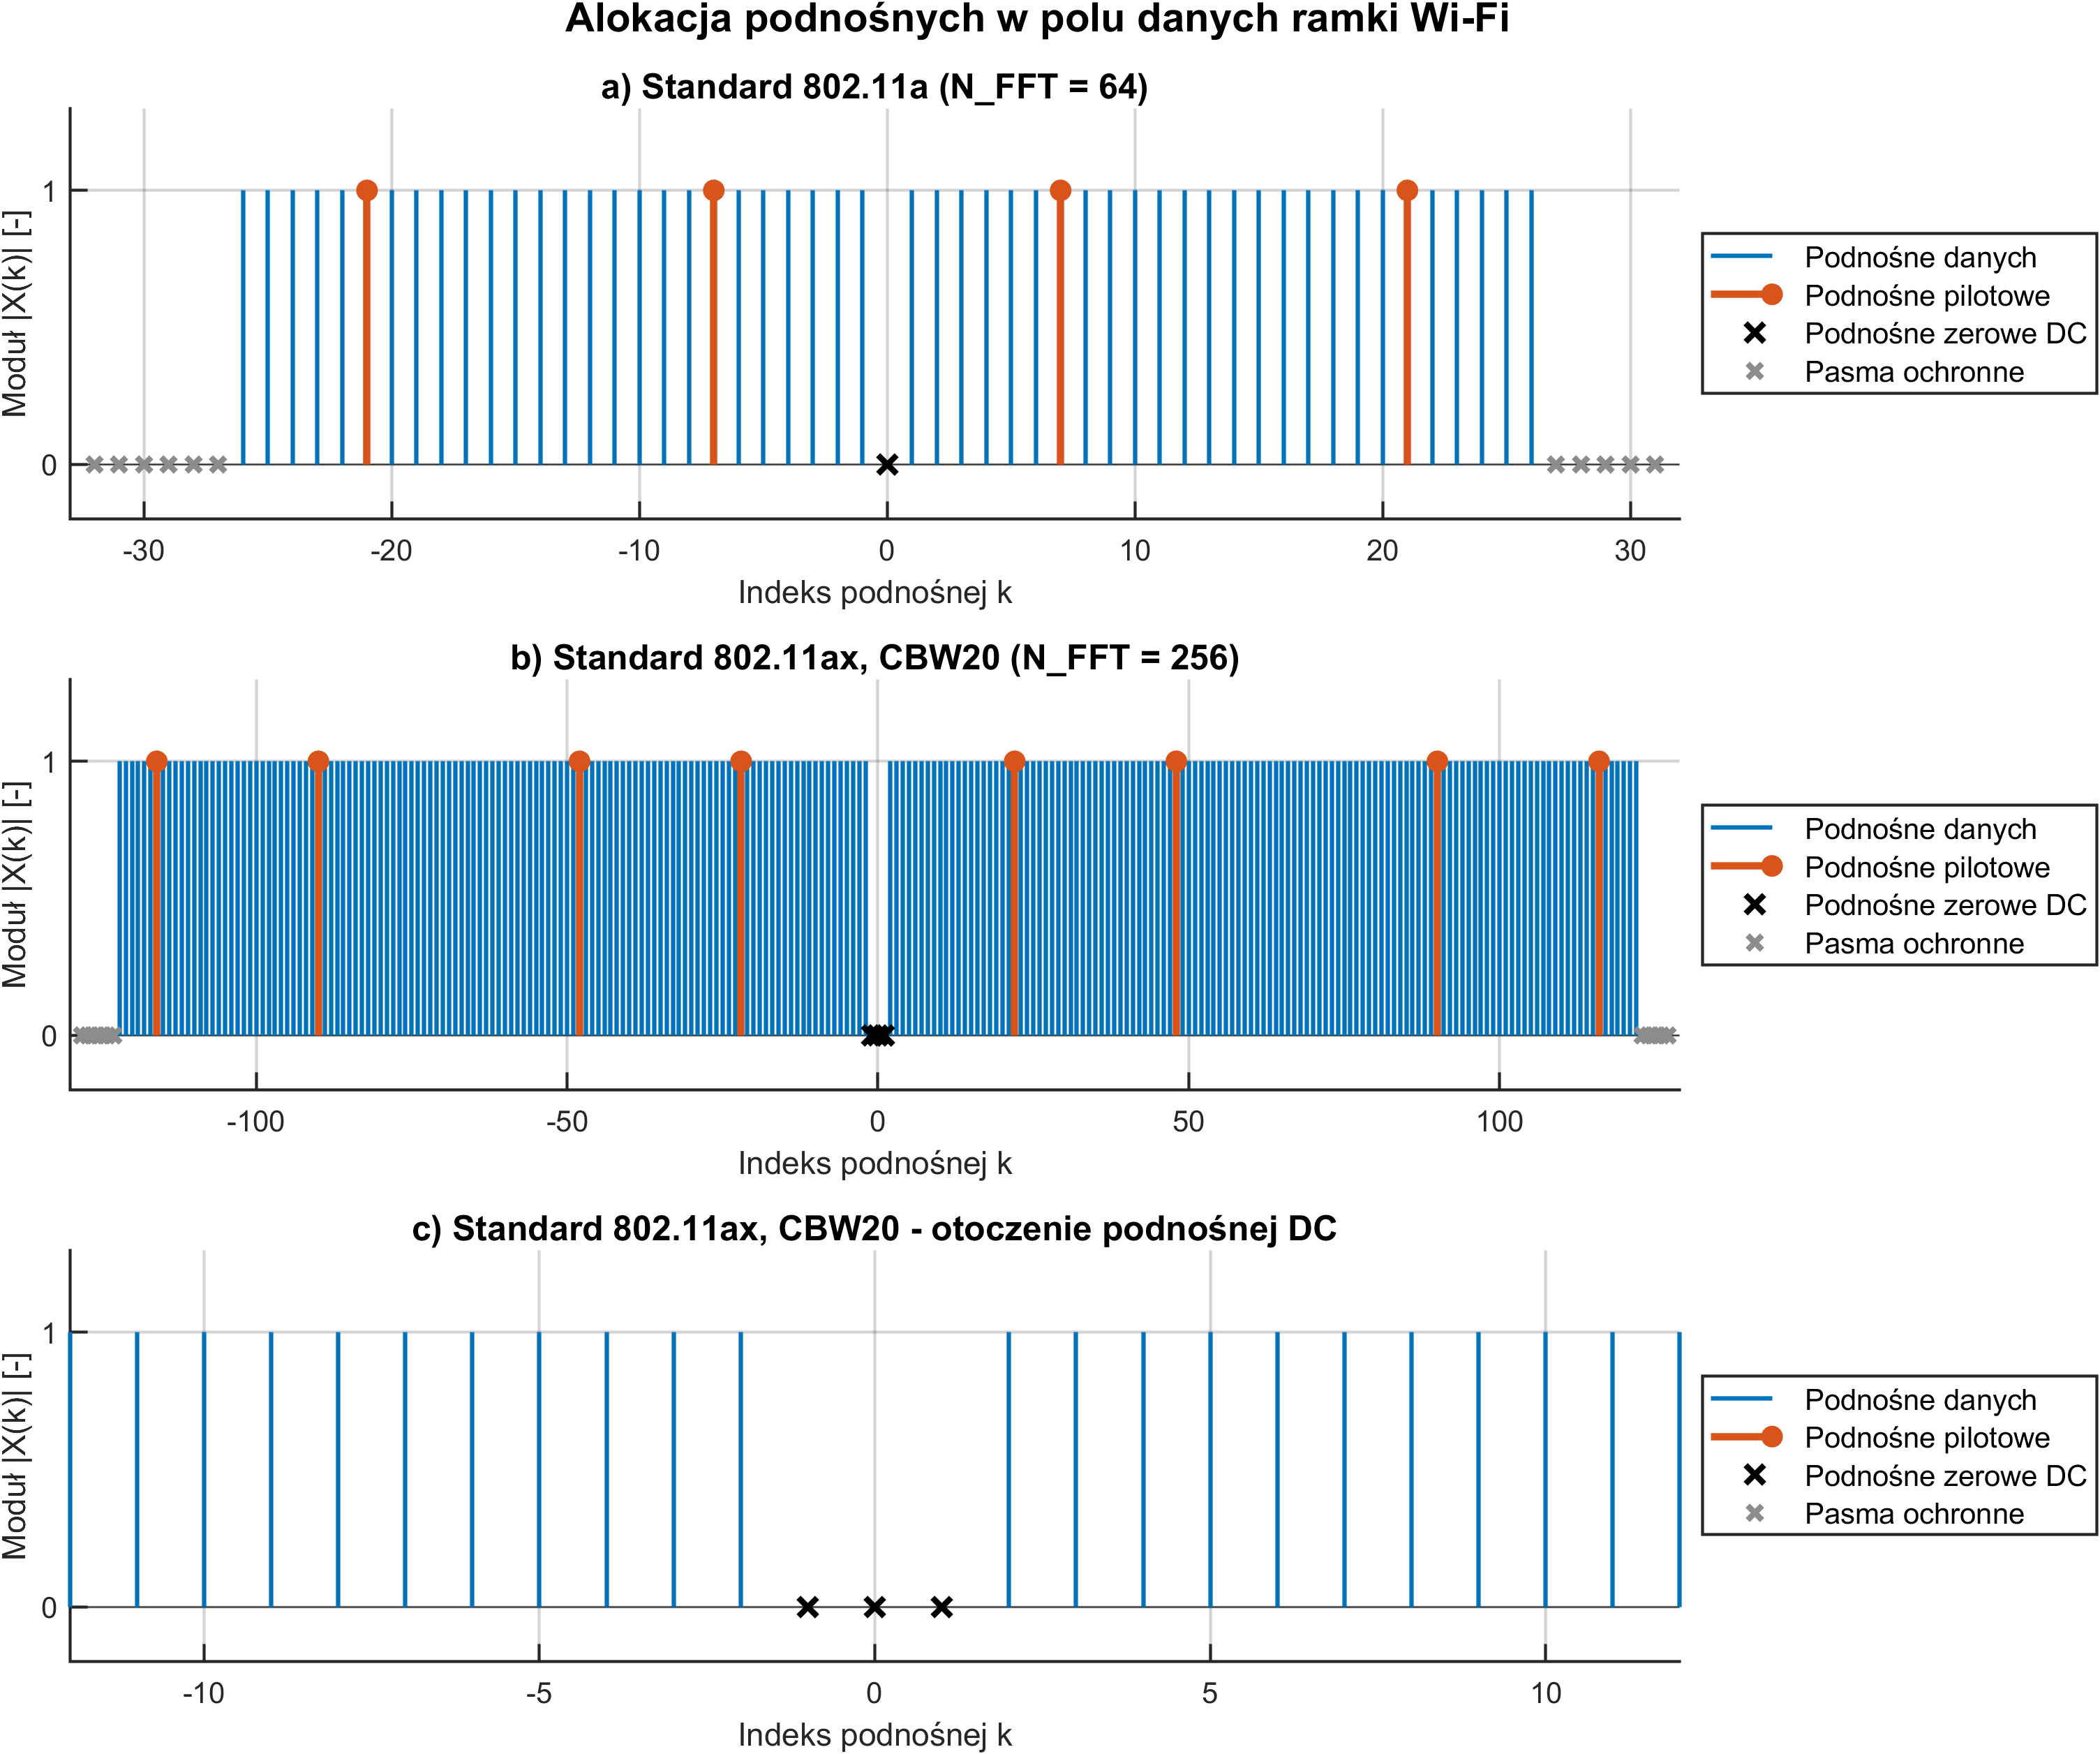
\includegraphics[width=\textwidth]{img/ch2_theory/rys_2_1_alokacja_podnosnych.png}
    \caption{Alokacja podnośnych w~polu danych: a)~802.11a, b)~802.11ax przy szerokości kanału 20~MHz, c)~powiększenie otoczenia podnośnej DC w~802.11ax. Podnośne zerowe zaznaczono krzyżykami na poziomie zera}
    \label{fig:subcarrier_allocation}
\end{figure}

Rozkład podnośnych w~paśmie przedstawiono na rysunku~\ref{fig:subcarrier_allocation}. W~standardzie 802.11a aktywne są 52 z~64 podnośnych, a~w~802.11ax przy szerokości kanału 20~MHz wykorzystywane są 242 z~256 podnośnych. Podnośne pilotowe służą odbiornikowi komunikacyjnemu do śledzenia fazy i~zajmują ściśle określone pozycje w~siatce częstotliwościowej. Skrajne podnośne pozostawiono puste jako pasma ochronne, ograniczające emisję poza przydzielonym kanałem. Wyzerowano również podnośną centralną $k = 0$ (w~802.11ax wraz z~sąsiednimi $k = \pm 1$, co pokazano na rysunku~\ref{fig:subcarrier_allocation}c). W~odbiornikach radiowych na zerowej częstotliwości pośredniej naturalnie powstaje silny prążek zakłóceń od napięcia stałego oraz wewnętrznego oscylatora -- brak transmisji na tych podnośnych zapobiega więc zniekształceniu danych.

Alokacja podnośnych przenosi się bezpośrednio na właściwości wyznaczanej mapy odległość--prędkość:
\begin{itemize}
    \item Pasma ochronne ograniczają efektywnie zajęte pasmo do ok.~16,6~MHz w~802.11a oraz 19,1~MHz w~802.11ax, co determinuje rozdzielczość odległościową (podrozdział~\ref{subsec:pbr_fundamentals}).
    \item Wyzerowane podnośne DC tworzą nieciągłość (dziurę) w~środku widma, co po transformacji Fouriera podnosi tło listków bocznych w~osi odległości \cite[rozdz.~3.3.8]{braun2014}. Problem ten rozwiązuje interpolacja opisana w~podrozdziale~\ref{subsec:clutter_filtering}.
    \item Zmienna amplituda punktów konstelacji QAM w~polu danych powoduje wzmocnienie szumu estymaty kanału przy dzieleniu Zero-Forcing, co szczegółowo przeanalizowano w~podrozdziale~\ref{subsec:channel_estimation} i~zbadano w~podrozdziale~\ref{subsec:sim_mcs_noise_enhancement}.
    \item Czterokrotnie mniejszy odstęp podnośnych w~802.11ax wydłuża czas trwania symbolu z~4,0 do 13,6~$\mu$s. Zwiększa to zasięg jednoznaczny, lecz proporcjonalnie obniża maksymalną jednoznaczną prędkość radaru (podrozdział~\ref{subsec:pbr_fundamentals}).
\end{itemize}

\subsection{Modulacja OFDM}
\label{subsec:ofdm_modulation}

\subsection{Podstawy radaru pasywnego}
\label{subsec:pbr_fundamentals}

\subsection{Estymacja kanału}
\label{subsec:channel_estimation}

\subsection{Filtracja ech stałych}
\label{subsec:clutter_filtering}

\subsection{Wyznaczanie mapy Range--Doppler}
\label{subsec:range_doppler_map}

\subsection{Detekcja i ekstrakcja celów}
\label{subsec:target_detection_extraction}
